\label{sec:processing}
Die Signalsequenzen durchlaufen eine Verarbeitungskette (Abb. \ref{fig:data_processing_chain}) mit den Schritten Bandpassfilterung, Artefaktentfernung, Normalisierung, Fouriertransformation und Aufteilung nach Frequenzbändern.

\begin{figure}[h] 
  \begin{center}
    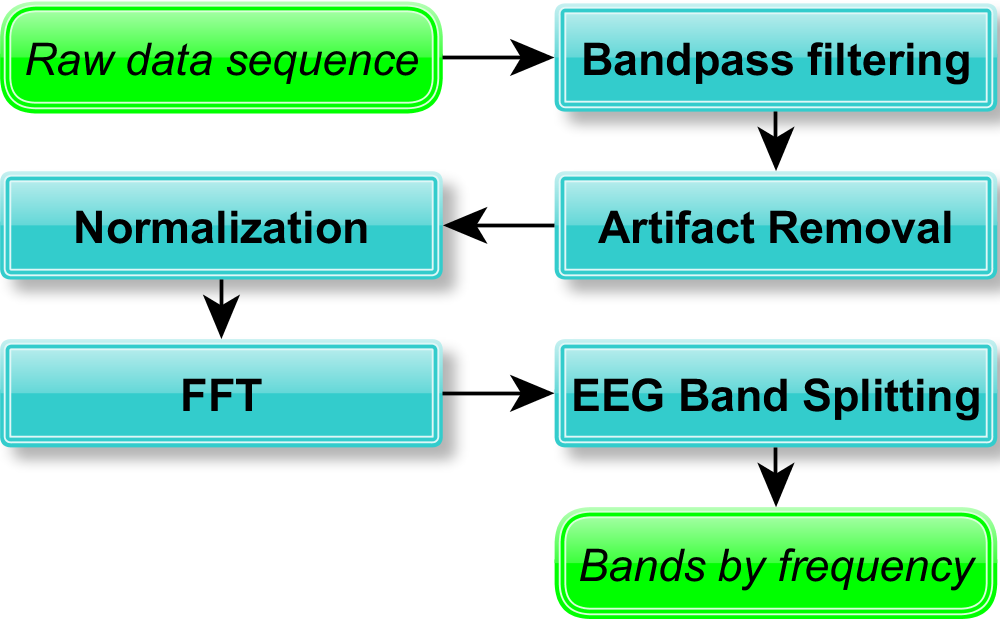
\includegraphics[width=5.5cm]{data_processing_chain}
    \caption[Verarbeitungskette]{Die Signalsequenzen durchlaufen eine Verarbeitungskette \label{fig:data_processing_chain}}
  \end{center}
\end{figure}

Um Störungen zu eliminieren wurde das Signal zu Beginn außerhalb des Bereichs von 0.53Hz - 50Hz eliminiert. Dies war eine Empfehlung aus einer Antwort auf ResearchGate \cite{resGate} und zeigt bei Tests gute Ergebnisse. Der Bandpassfilter zentrierte das Signal zudem. 

Für die Anwendung wurde hierfür ein Buttworth-Filter\cite{Butterworth30} eingesetzt. Gleichung \ref{eq:butterworth} zeigt die Übertragungsfunktion mit $A_0$: Gleichspannungsverstärkung, $\Omega = \frac{f}{f_g}$: auf Grundfrequenz normierte Frequenz und $n$: Ordnung des Filters. Abbildung \ref{fig:butterworth_filter} zeigt exemplarisch Filterfunktionen verschiedener Ordnung mit den Grenzen von 500 bis 1250Hz. Alle Frequenzen darunter und darüber werden deutlich abgeschwächt bzw. gehen gegen null. Der Butterworth-Filter verläuft nahe Eins im gewünschten Bereich, fällt an den Grenzen ab und stellt sicher, dass das Signal an den Grenzen um $\frac{1}{\sqrt{2}} \approx 0.7071$ gemindert wird. Je höher die Ordnung, desto steiler geht die Funktion durch die angegebenen Grenzen. Der Filter lässt sich gut in Hardware realisieren.

\begin{equation} \label{eq:butterworth}
\left|\underline{A}\right|^2 = \frac{A_0^2}{1+ k_{2n} \Omega ^{2n}}
\end{equation}

\begin{figure}[h] 
  \begin{center}
    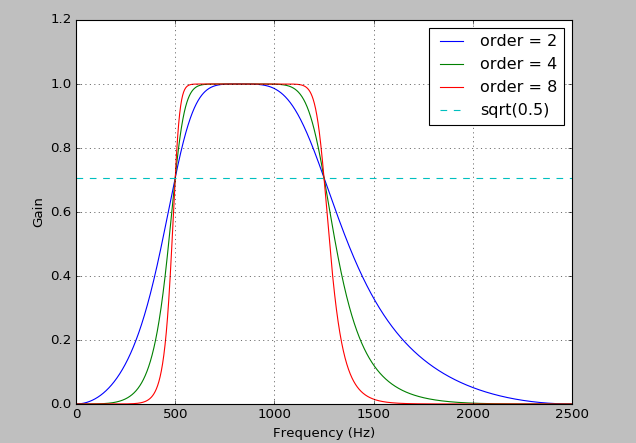
\includegraphics[width=5.5cm]{butterworth_filter}
    \caption[Butterworth-Filter]{Die Filterfunktion eines Butterworthfilters 2., 4,. und 8. Ordnung im Frequenzbereich von 500 bis 1250Hz. \label{fig:butterworth_filter}}
  \end{center}
\end{figure}

Bei der Analyse der Histogramme der Signalwerte, zeigte sich eine Häufung der Amplituden im Bereich von -100 bis 100 (siehe Abb. \ref{fig:raw_histo}). Außerhalb dieses Bereichs wurde als Artefakte angesehen und herausgefiltert (als ungültig markiert).

\begin{figure}[h] 
  \begin{center}
    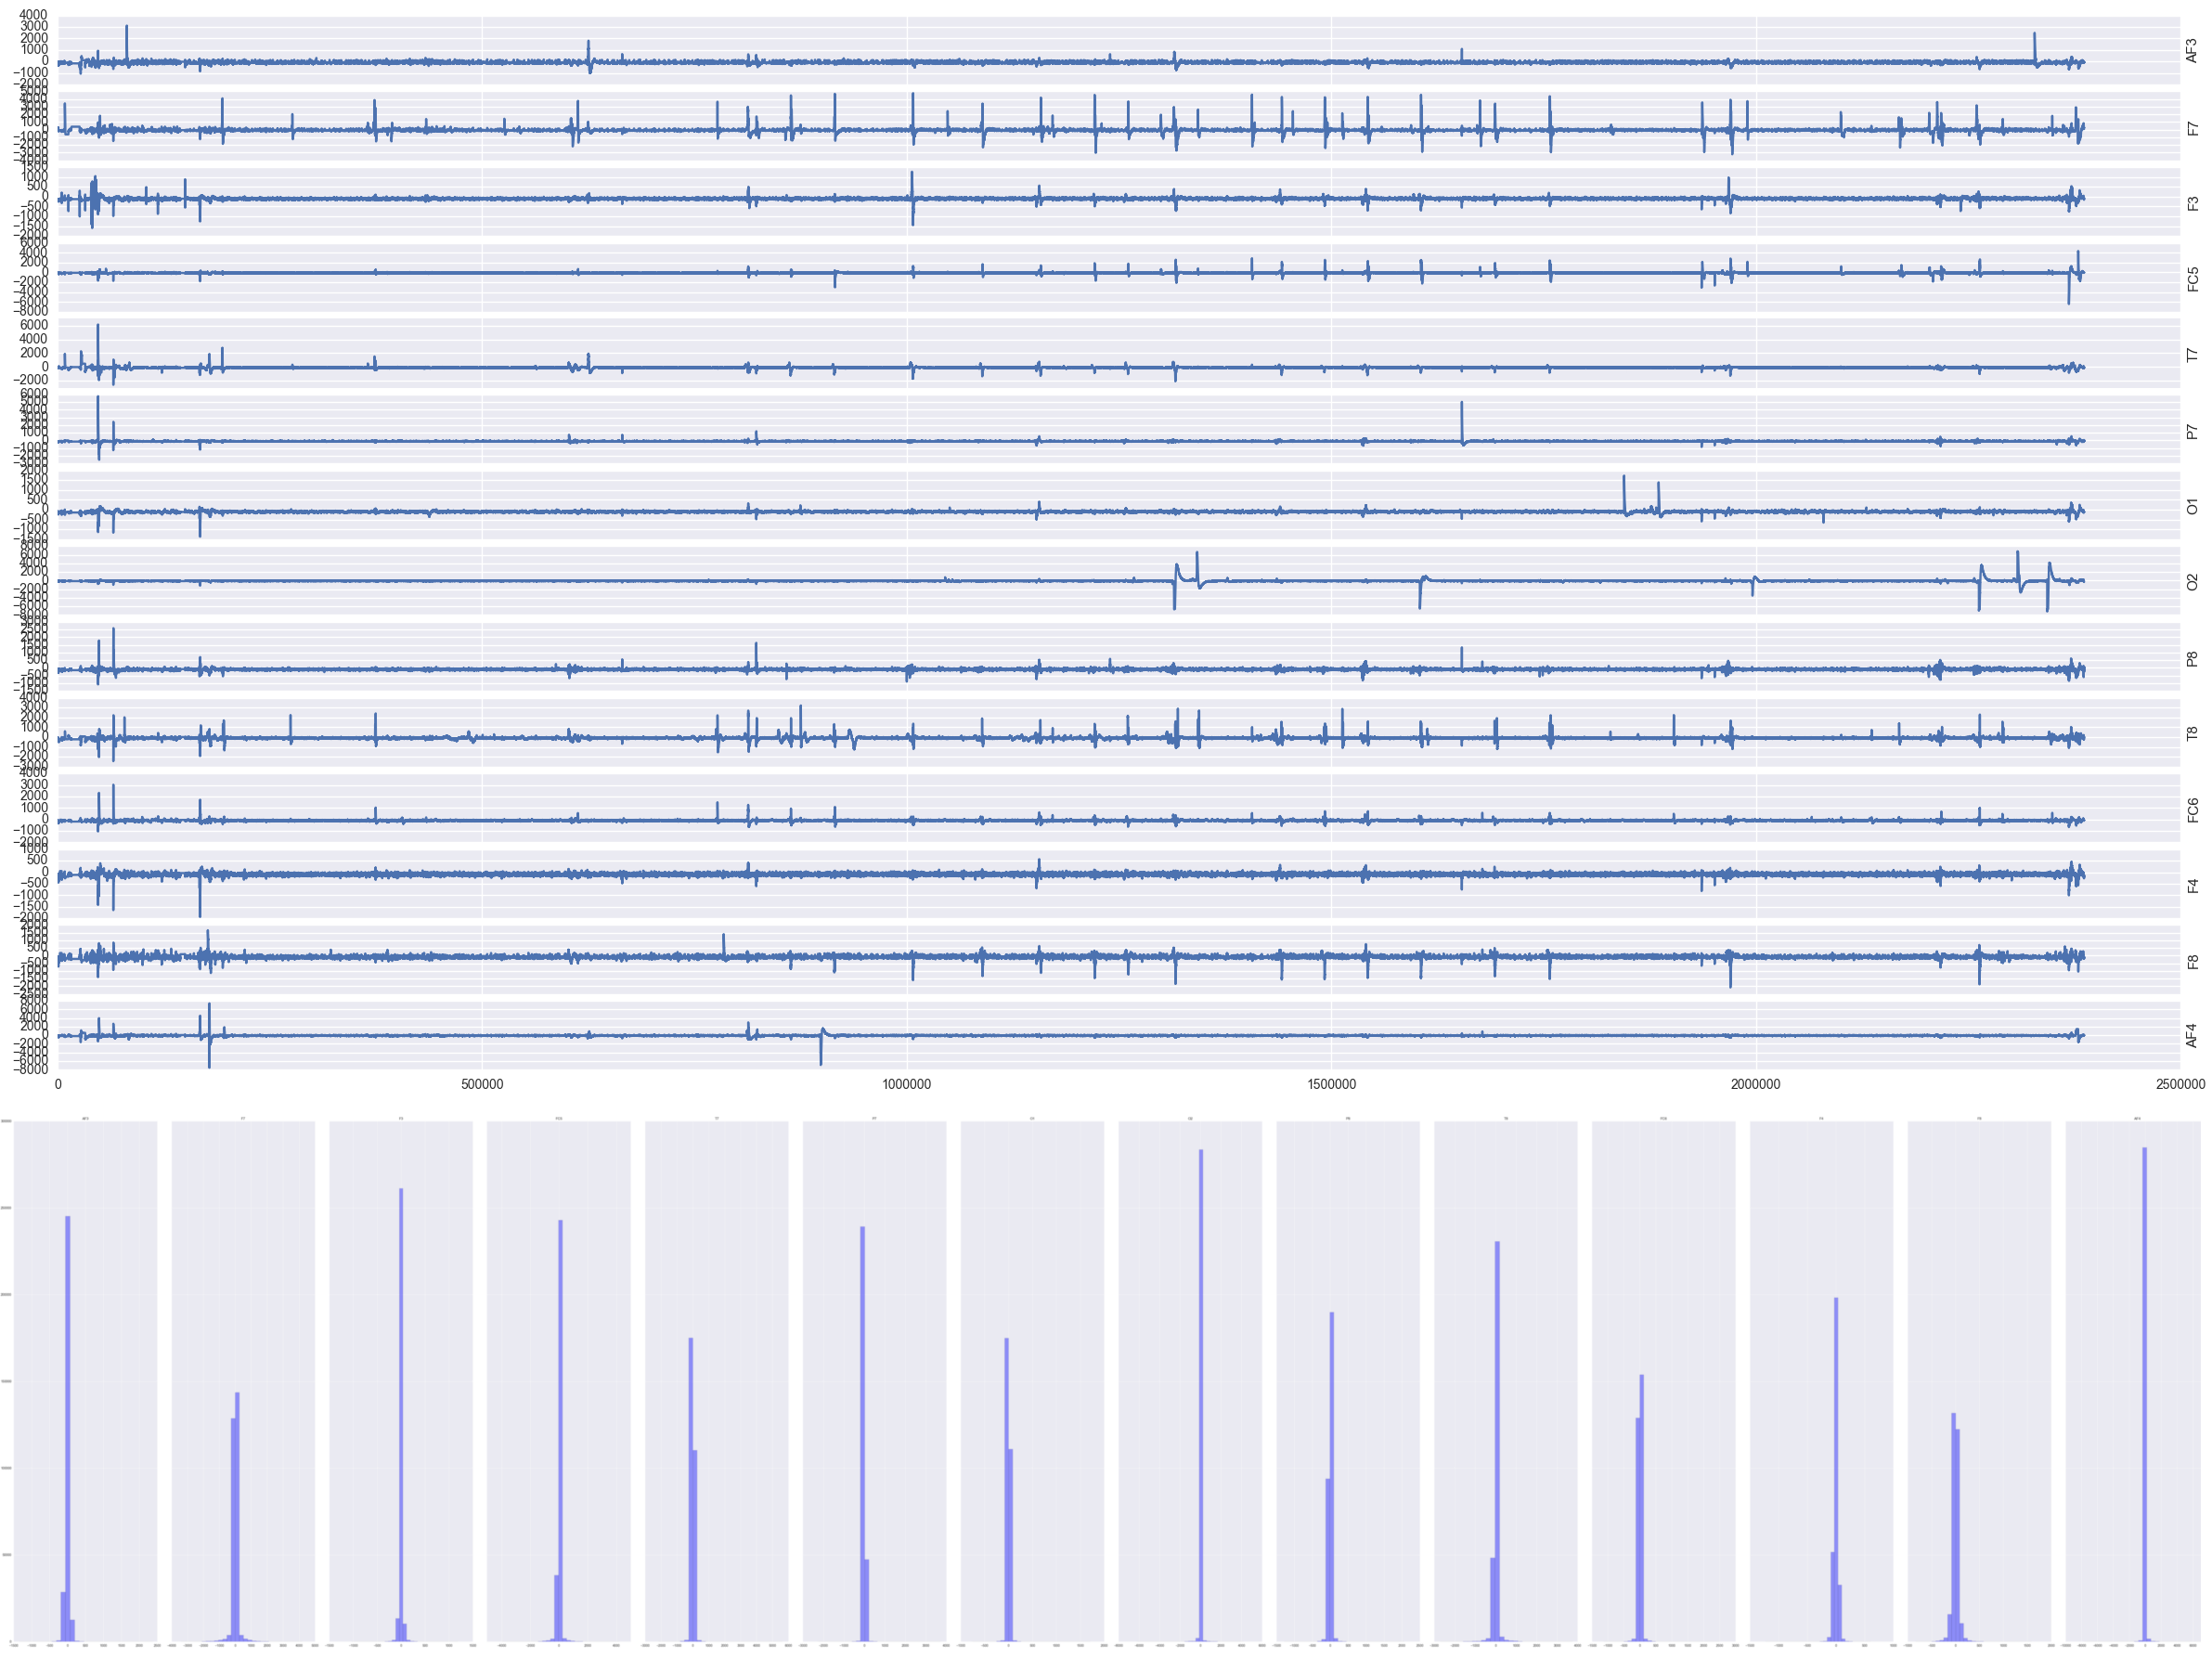
\includegraphics[width=\docwidth]{raw_histo}
    \caption[Rohsignal und Histogramm]{Die Rohsignale pro Sensore und das dazugehörige Histogramm. Die Werte verteilen sich zwischen -8000 bis 8000, ein deutliches Maximum im Histogramm ist zwischen -100 und 100 erkennbar.  \label{fig:raw_histo}}
  \end{center}
\end{figure}

Die gefilterten Signal werden dann auf einen Bereich von -1 bis 1 normalisiert, dazu werden die Signale durch den jeweiligen Maximalwert bzw. Betrag des Minimalwertes geteilt (In diesem Fall 100). Dieses Vorgehen stellt sicher, dass die absolute Amplitude keinen Einfluss auf die Gewichtung im Klassifikator hat. Zudem wird die Datenmenge wiederum reduziert. Im letzten Schritt werden die Signale in ihre Frequenzbänder (EEG-Bänder) unterteilt. Hierzu werden die Signale in ihr Frequenzspektrum zerlegt und bestimmte Frequenzbereiche extrahiert. Diese EEG-Bänder gliedern sich in folgende Frequenzbereiche und werden nach griechischen Buchstaben benannt:
\begin{itemize}
 \item $\delta$ : 0,1 bis < 4Hz
 \item $\theta$ :   4 bis < 8Hz
 \item $\alpha$ :   8 bis < 13Hz
 \item $\beta$  :  13 bis < 30Hz
 \item $\gamma$ :  > 30Hz
\end{itemize}
Die Frequenzbereiche sind nicht einheitlich definiert und variieren unter Umständen. Die Frequenzbereich sind aus Empfehlungen der IFCN entnommen \cite{ifcn}. Den Frequenzbändern werden verschiedene Eigenschaften zugesprochen \cite{lei2011,Lv2010,Gundel1992}. Delta Wellen treten bei Erwachsenen häufig in der traumlosen Tiefschlafphase auf. Theta-Wellen zeigen sich bei Schläfrigkeit und leichtem Schlaf. Mit leichter Entspannung und entspannter Wachheit (mit geschlossenen Augen) werden Alpha-Wellen assoziiert. Beta Wellen treten während der REM-Schlafphase oder unter Einwirkung von Psychopharmaka auf. Gamma-Wellen gehen häufig mit starker Konzentration oder Meditation einher.

Um die einzelnen Frequenzbänder zu erhalten wird eine Fast-Fourier-Transformation \cite{Bochner_1} durchgeführt. Alternativ wäre auch ein Wavelet-Transformation \cite{Chui:1992:IW:163196} möglich gewesen. Beide Ansätze fanden sich in der Literatur Recherche, aus Zeitgründen wurde auf einen Vergleich der Ansätze verzichtet. 
Die Fourier-Transformation bildet ein zeitdiskretes endliches Signal, auf ein diskretes, periodisches Frequenzspektrum ab (siehe Abb. \ref{fig:fft_example}). Um die Frequenzbänder zu erhalten, wird das Ergebnis auf die gewünschten Frequenzen reduziert.

\begin{figure}[h] 
  \begin{center}
    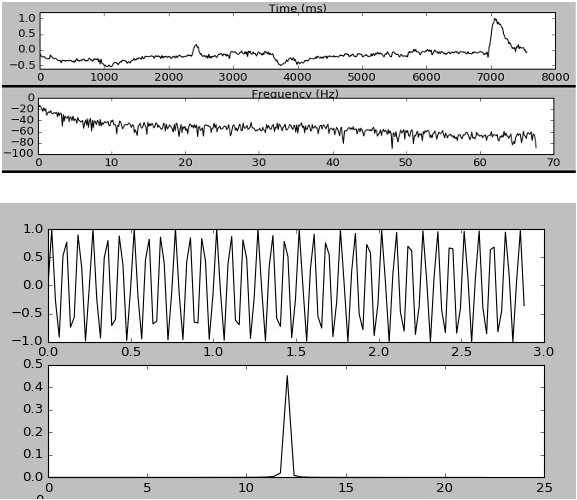
\includegraphics[width=\docwidth]{fft_example}
    \caption[Fast Fourier Transformation]{Oben: EEG Signal darunter das Frequenzspektrum. Unten: die selbe Anordnung nur für ein Tonsignal, das Tonsignal schwingt mit 12KHz, dies zeigt sich durch ein Maximum bei dieser Frequenz. \label{fig:fft_example}}
  \end{center}
\end{figure}
